\documentclass[10pt,a4paper]{article}
\usepackage[utf8]{inputenc}
\usepackage[T1]{fontenc}
\usepackage{lmodern}
\usepackage[margin=1.5cm, top=1.4cm, bottom=1.4cm]{geometry}
\usepackage{hyperref}
\usepackage{enumitem}
\usepackage{titlesec}
\usepackage{xcolor}
\usepackage{graphicx}

\definecolor{accent}{HTML}{00686E}
\hypersetup{colorlinks=true, urlcolor=accent, linkcolor=accent}
\pagenumbering{arabic}
\setlength{\parindent}{0pt}

\titleformat{\section}{\large\bfseries\color{accent}}{}{0em}{}[\vspace{-0.6em}\rule{\textwidth}{0.8pt}]
\titlespacing{\section}{0pt}{7pt}{4pt}

\newcommand{\role}[4]{%
  \textbf{#1} \hfill \textbf{#2}\\[1pt]%
  \textit{#3} \hfill \textit{#4}\\[2pt]%
}
\setlist[itemize]{leftmargin=1.2em, itemsep=1.5pt, topsep=2pt, parsep=0pt}

\begin{document}

% ================= HEADER =================
\begin{minipage}[c]{0.80\textwidth}
  {\Huge\bfseries Prabhavit Gupta}\\[3pt]
  {\color{accent}\large AI Solutions Engineer: LLM Applications, MCP Integrations \& Internal Automation}\\[6pt]
  {\footnotesize +39 351 610 7807 ~$\vert$~
  \href{mailto:prabhavitg@gmail.com}{prabhavitg@gmail.com} ~$\vert$~
  \href{https://www.linkedin.com/in/prabhavit/}{linkedin.com/in/prabhavit} ~$\vert$~
  \href{https://github.com/prab-gupta}{github.com/prab-gupta} ~$\vert$~
  Venice, Italy}
\end{minipage}\hfill
\begin{minipage}[c]{0.18\textwidth}
  \raggedleft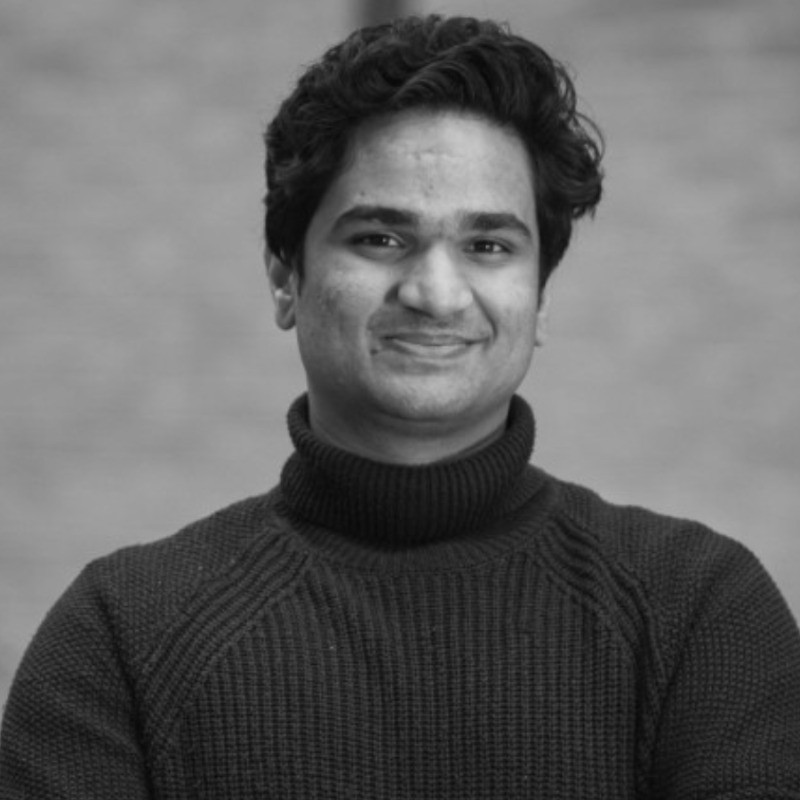
\includegraphics[width=2.0cm]{photo.jpg}
\end{minipage}
\vspace{-2pt}

% ================= SUMMARY =================
\section{Summary}
AI Solutions Engineer and Automation Developer with 3 years of hands-on experience designing and deploying production LLM tools, agent architectures, and autonomous internal automations. Daily power-user of AI coding agents (Claude Code) as a default operating mode to rapidly take solutions from problem definition to live adoption in days. Proven track record building ad-hoc document processing pipelines, RAG systems, structured data extraction, and deep API/MCP connectors across CRM, databases, and operational business platforms. Highly autonomous builder who collaborates directly with cross-functional business teams (Finance, Operations, Support, Legal) to analyze real workflows and ship practical, user-adopted tools. Based in Venice, Italy with an EU Long Term Residence Permit (unrestricted EU work authorization without sponsorship). Immediately available.

% ================= TECHNICAL EXPERTISE =================
\section{Technical Expertise}
\begin{itemize}
  \item \textbf{AI \& LLM Engineering:} Production LLM toolchains (Claude API, OpenAI), Prompt engineering, Structured JSON outputs, Function calling, Tool use, RAG, Model error handling \& evaluation, Context window management.
  \item \textbf{Autonomous Development \& AI Tooling:} Daily default workflow using Claude Code and modern AI coding agents for high-speed end-to-end prototyping, implementation, and refactoring.
  \item \textbf{Integrations \& Automation:} REST APIs, Webhook architectures, MCP (Model Context Protocol) connectors, n8n workflow orchestration, Zapier/Make, Database syncs (PostgreSQL, Supabase), Rate-limiting \& retries.
  \item \textbf{Core Languages \& Stack:} TypeScript, JavaScript, Python, SQL, Next.js, Node.js, Git version control, Postman.
  \item \textbf{Business Workflow Automation:} Rapid translation of cross-functional team processes (Operations, HR, Finance, Support) into automated tools, user training, and direct handoff to production.
  \item \textbf{Languages \& Work Authorization:} Hindi (Native), English (C1 Professional), Italian (Beginner). EU Long Term Residence Permit (Permanent unrestricted EU work authorization; no visa sponsorship required).
\end{itemize}

% ================= EXPERIENCE =================
\section{Experience}

\role{\href{https://flowspace.co}{FlowSpace.co}}{Mar 2024 - Aug 2026}{Lead Developer (Full-time, Freelance)}{London, UK (remote)}
\begin{itemize}
  \item Built and deployed custom LLM-powered internal tools and automated pipelines that processed unstructured partner data into structured formats, scaling platform listings to 900+ active records.
  \item Integrated core operational platforms (OfficeRnD, Nexudus, CRM) via bi-directional REST APIs and webhooks, automating lead ingestion, scheduling, and customer data reconciliation.
  \item Engineered AI support and triage agents using Claude API and structured output schemas, reducing manual ticket resolution time for customer operations teams.
  \item Spearheaded migration of the core platform from a legacy stack to a modern Next.js and Laravel architecture, scaling the active user base from 2,000 to 4,500+ users.
  \item Leveraged Claude Code daily to rapidly prototype, iterate, and deliver production-ready features in days rather than multi-week sprints.
  \item Designed and executed comprehensive automated test suites using Playwright, verifying continuous integration stability and preventing regressions across business workflows.
  \item Partnered directly with non-technical business teams to analyze manual bottlenecks, author comprehensive operational documentation, and guide end-user adoption.
\end{itemize}

\role{Urlink}{Apr 2025 - Jul 2025}{Project Manager \& AI Assisted Developer (Freelance)}{Barcelona, Spain (remote)}
\begin{itemize}
  \item Delivered web application integration features and internal tools by scoping business logic, defining API schemas, and implementing automated data transformation services.
  \item Built automated pipelines connecting external service APIs with relational databases, ensuring strict schema validation and reliable error handling.
  \item Configured CI/CD workflows and automated quality checks, accelerating release velocity while maintaining zero downtime.
\end{itemize}

\role{Independent Technical Consultant}{Aug 2023 - Feb 2024}{AI Solutions \& Automation Engineer}{Venice, Italy}
\begin{itemize}
  \item Designed and shipped bespoke AI automations, web extraction tools, and API connectors for European SME clients using Python, TypeScript, and Playwright.
  \item Audited operational workflows across sales, finance, and support to identify high-leverage automation opportunities, delivering practical tools adopted directly by non-technical staff.
  \item Built webhook listeners and automated data reconciliation scripts that eliminated manual data entry across disparate SaaS tools.
\end{itemize}

% ================= EDUCATION =================
\section{Education}
\role{Ca' Foscari University of Venice}{2020 - 2024}{BA in Philosophy, International Studies and Economics}{Venice, Italy}
\begin{itemize}
  \item Rigorous training in formal logic, analytical problem solving, systems analysis, and macroeconomic decision models.
\end{itemize}

\end{document}
